%%%%%%%%%%%%%%%%%%%%%%%%%%%%%%%%%%%%%%%%%%%%%%%%%%%%%%%%%%%%%%%%%%%%%%%%
\chapter{D'AlemBERT}
%%%%%%%%%%%%%%%%%%%%%%%%%%%%%%%%%%%%%%%%%%%%%%%%%%%%%%%%%%%%%%%%%%%%%%%%

\section{Carbon Footprint}\label{carbon-footprint-dalembert}

\begin{table}[th]
    \centering\small
    \begin{tabular}{lrrrr}
        \toprule
        \textbf{Model}               & {\textbf{Power (W)}} & {\textbf{Time (h)}} & {\textbf{(PUE$\cdotp$kWh)}} & {\textbf{CO\textsuperscript{2}e (kg)}} \\
        \midrule
        Pre-train                    & 48640                & 20                  & 1537.02                     & 46.11                                  \\
        Evaluation                   & 589                  & 1                   & 0.93                        & 0.03                                   \\
        \midrule
        Total CO\textsuperscript{2}e &                      &                     &                             & 46.14                                  \\
        \bottomrule
    \end{tabular}
    \caption{Average power draw, number of models trained, training times in hours, mean power consumption including power usage effectiveness (PUE), and CO\textsuperscript{2} emissions; for each setting.}
    \label{tab:carbon-dalembert}
\end{table}

In light of recent interest concerning the energy consumption and carbon emission of machine learning models and specifically of those of language models \cite{schwartz-etal-2020-green,bender-etal-2021-on}, we have decided to report the power consumption and carbon footprint of all our experiments following the approach of \newcite{strubell-etal-2019-energy}. We report the energy consumption and carbon emissions of both the pre-training of D'AlemBERT and its evaluation.

\paragraph{Pre-training:} We use a cluster of 32 machines, each one having 4 GPU Nvidia Tesla V100 SXM2 32GiB, 192GiB of RAM, and two Intel Xeon Gold 6248 processors. One Nvidia Tesla V100 card is rated at around 300W,\footnote{\href{https://www.nvidia.com/en-us/data-center/v100/}{ Nvidia Tesla V100 specification}} while the Xeon Gold 6248 processor is rated at 150W.\footnote{\href{https://ark.intel.com/content/www/us/en/ark/products/192446/intel-xeon-gold-6248-processor-27-5m-cache-2-50-ghz.html}{Intel Xeon Gold 6248 specification}} For the DRAM we can use the work of \newcite{desrochers-etal-2016-a} to estimate the total power draw of 192GiB of RAM at around 20W. Thus, the total power draw of the pre-training adds up to around 48640W.

\paragraph{Evaluation:} We use a single machine with a single GPU Nvidia Tesla V100 SXM2 32GiB, 384GiB of RAM and two Intel Xeon Gold 6226 processors. The Xeon Gold 6226 processor is rated at 125 W,\footnote{\href{https://ark.intel.com/content/www/us/en/ark/products/193957/intel-xeon-gold-6226-processor-19-25m-cache-2-70-ghz.html}{Intel Xeon Gold 6226 specification}} and the DRAM total power draw can be estimated at around 39W. Therefore, the total power draw of the evaluation adds up to around 589W.

With this information, we use the formula proposed by \newcite{strubell-etal-2019-energy} to compute the total power required for each setting:

\begin{equation*}
    p_t = \frac{1.58t(cp_{c} + p_r + gp_g)}{1000}
\end{equation*}

Where $c$ and $g$ are the number of CPUs and GPUs respectively, $p_c$ is the average power draw (in W) from all CPU sockets, $p_r$ the average power draw from all DRAM sockets and $p_g$ the average power draw of a single GPU. We estimate the total power consumption by adding GPU, CPU and DRAM consumption, and then multiplying by the \emph{Power Usage Effectiveness} (PUE), which accounts for the additional energy required to support the compute infrastructure. We use a PUE coefficient of 1.58, the 2018 global average for data centers \cite{strubell-etal-2019-energy}. In Table~\ref{tab:carbon-dalembert} we report the training times in hours, as well as the total power draw (in Watts) of the system used to train the models. We use this information to compute the total power consumption of each setting, also reported in Table~\ref{tab:carbon-dalembert}.

We can further estimate the CO\textsuperscript{2} emissions in kilograms of each single model by multiplying the total power consumption by the average CO\textsuperscript{2} emissions per kWh in our region, which were around 30g/kWh between the 30\textsuperscript{th} and the 31\textsuperscript{st} of December,\footnote{\href{https://www.rte-france.com/eco2mix/les-emissions-de-co2-par-kwh-produit-en-france}{Rte - éCO\textsuperscript{2}mix}.} when the models were trained. Thus the total CO\textsuperscript{2} emissions in kg for one single model can be computed as:

\begin{equation*}
    \text{CO}_{2}\text{e} = 0.030 p_t
\end{equation*}

All emissions are also reported in Table~\ref{tab:carbon-dalembert}.

\section{Detail Results of Experiments in NER by Entity Type}

Here we show the results of each of the trained NER models by entity type.

\begin{table}[ht!]
    \centering\small
    \begin{tabular}{lrrrr}
        \toprule
        \multicolumn{5}{c}{\textsc{LSTM-CRF}}                  \\
        \midrule
        Entity Type  & Precision & Recall & F1-Score & Support \\
        \midrule
        pers         & 0.8808    & 0.8435 & 0.8617   & 2734    \\
        loc          & 0.8109    & 0.8707 & 0.8397   & 1384    \\
        amount       & 0.9040    & 0.9040 & 0.9040   & 250     \\
        time         & 0.9604    & 0.9237 & 0.9417   & 236     \\
        func         & 0.8872    & 0.8429 & 0.8645   & 140     \\
        org          & 0.8824    & 0.6122 & 0.7229   & 49      \\
        prod         & 0.9231    & 0.4444 & 0.6000   & 27      \\
        event        & 0.7273    & 0.6667 & 0.6957   & 12      \\
        \midrule
        micro avg    & 0.8640    & 0.8533 & 0.8586   & 4832    \\
        macro avg    & 0.8720    & 0.7635 & 0.8038   & 4832    \\
        weighted avg & 0.8659    & 0.8533 & 0.8583   & 4832    \\
        samples avg  & 0.7737    & 0.7737 & 0.7737   & 4832    \\
        \bottomrule
    \end{tabular}
    \caption{Results of the BiLSTM-CRF model on the test set of \freemner by entity type.}
\end{table}

\begin{table}[ht!]
    \centering\small
    \begin{tabular}{lrrrr}
        \toprule
        \multicolumn{5}{c}{\textsc{CamemBERT}}                 \\
        \midrule
        Entity Type  & Precision & Recall & F1-Score & Support \\
        \midrule
        pers         & 0.9373    & 0.9236 & 0.9304   & 2734    \\
        loc          & 0.9140    & 0.9371 & 0.9254   & 1384    \\
        amount       & 0.9840    & 0.9840 & 0.9840   & 250     \\
        time         & 0.9447    & 0.9407 & 0.9427   & 236     \\
        func         & 0.9209    & 0.9143 & 0.9176   & 140     \\
        org          & 0.8364    & 0.9388 & 0.8846   & 49      \\
        prod         & 0.7742    & 0.8889 & 0.8276   & 27      \\
        event        & 0.8333    & 0.8333 & 0.8333   & 12      \\
        \midrule
        micro avg    & 0.9303    & 0.9309 & 0.9306   & 4832    \\
        macro avg    & 0.8931    & 0.9201 & 0.9057   & 4832    \\
        weighted avg & 0.9307    & 0.9309 & 0.9307   & 4832    \\
        samples avg  & 0.8856    & 0.8856 & 0.8856   & 4832    \\
        \bottomrule
    \end{tabular}
    \caption{Results of CamemBERT on the test set of \freemner by entity type.}
\end{table}

\begin{table}[ht!]
    \centering\small
    \begin{tabular}{lrrrr}
        \toprule
        \multicolumn{5}{c}{\textsc{D'AlemBERT}}                \\
        \midrule
        Entity Type  & Precision & Recall & F1-Score & Support \\
        \midrule
        pers         & 0.9355    & 0.9279 & 0.9317   & 2734    \\
        loc          & 0.9242    & 0.9335 & 0.9288   & 1384    \\
        amount       & 0.9800    & 0.9800 & 0.9800   & 250     \\
        time         & 0.9456    & 0.9576 & 0.9516   & 236     \\
        func         & 0.9333    & 0.9000 & 0.9164   & 140     \\
        org          & 0.8148    & 0.8980 & 0.8544   & 49      \\
        prod         & 0.8621    & 0.9259 & 0.8929   & 27      \\
        event        & 0.8333    & 0.8333 & 0.8333   & 12      \\
        \midrule
        micro avg    & 0.9329    & 0.9323 & 0.9326   & 4832    \\
        macro avg    & 0.9036    & 0.9195 & 0.9111   & 4832    \\
        weighted avg & 0.9331    & 0.9323 & 0.9327   & 4832    \\
        samples avg  & 0.8893    & 0.8893 & 0.8893   & 4832    \\
        \bottomrule
    \end{tabular}
    \caption{Results of D'AlemBERT model on the test set of \freemner by entity type.}
\end{table}

\section{Entity Distribution by Text in NER Data}

The following diagrams show the detail of the coarse entity distribution by text in \freemner.

\begin{sidewaysfigure}[!ht]
    \centering
    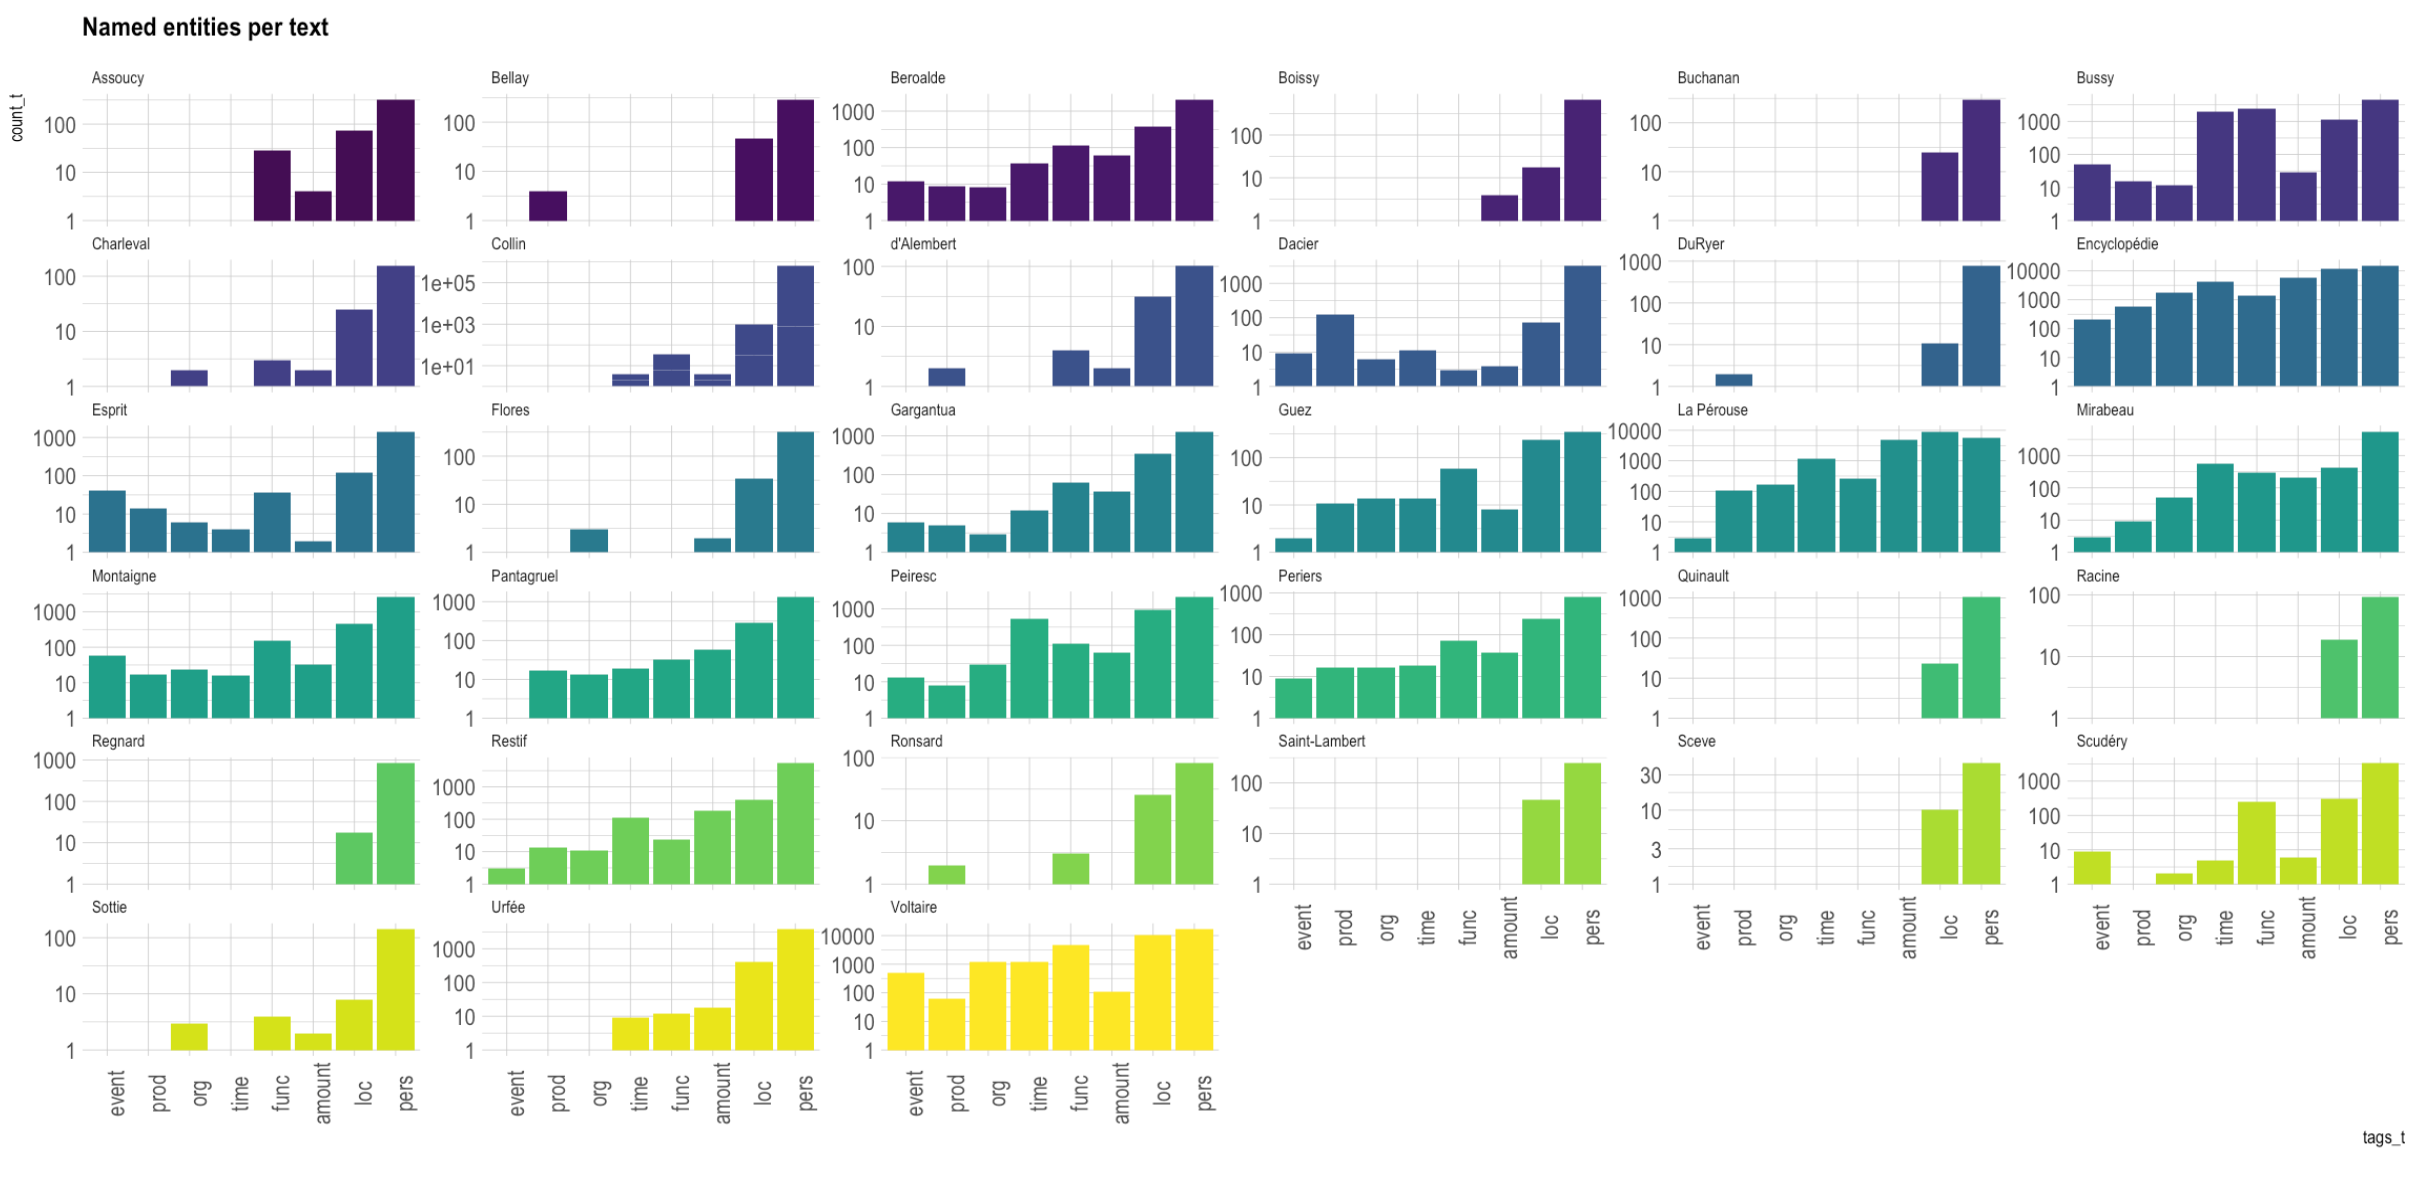
\includegraphics[width=\textwidth]{static/media/mod_eval/dalembert/freem_ner_entities_by_text.png}
    \caption{Number of entities by text on a logarithmic scale.}
    \label{fig:entities-by-text}
\end{sidewaysfigure}

\begin{sidewaysfigure}[!ht]
    \centering
    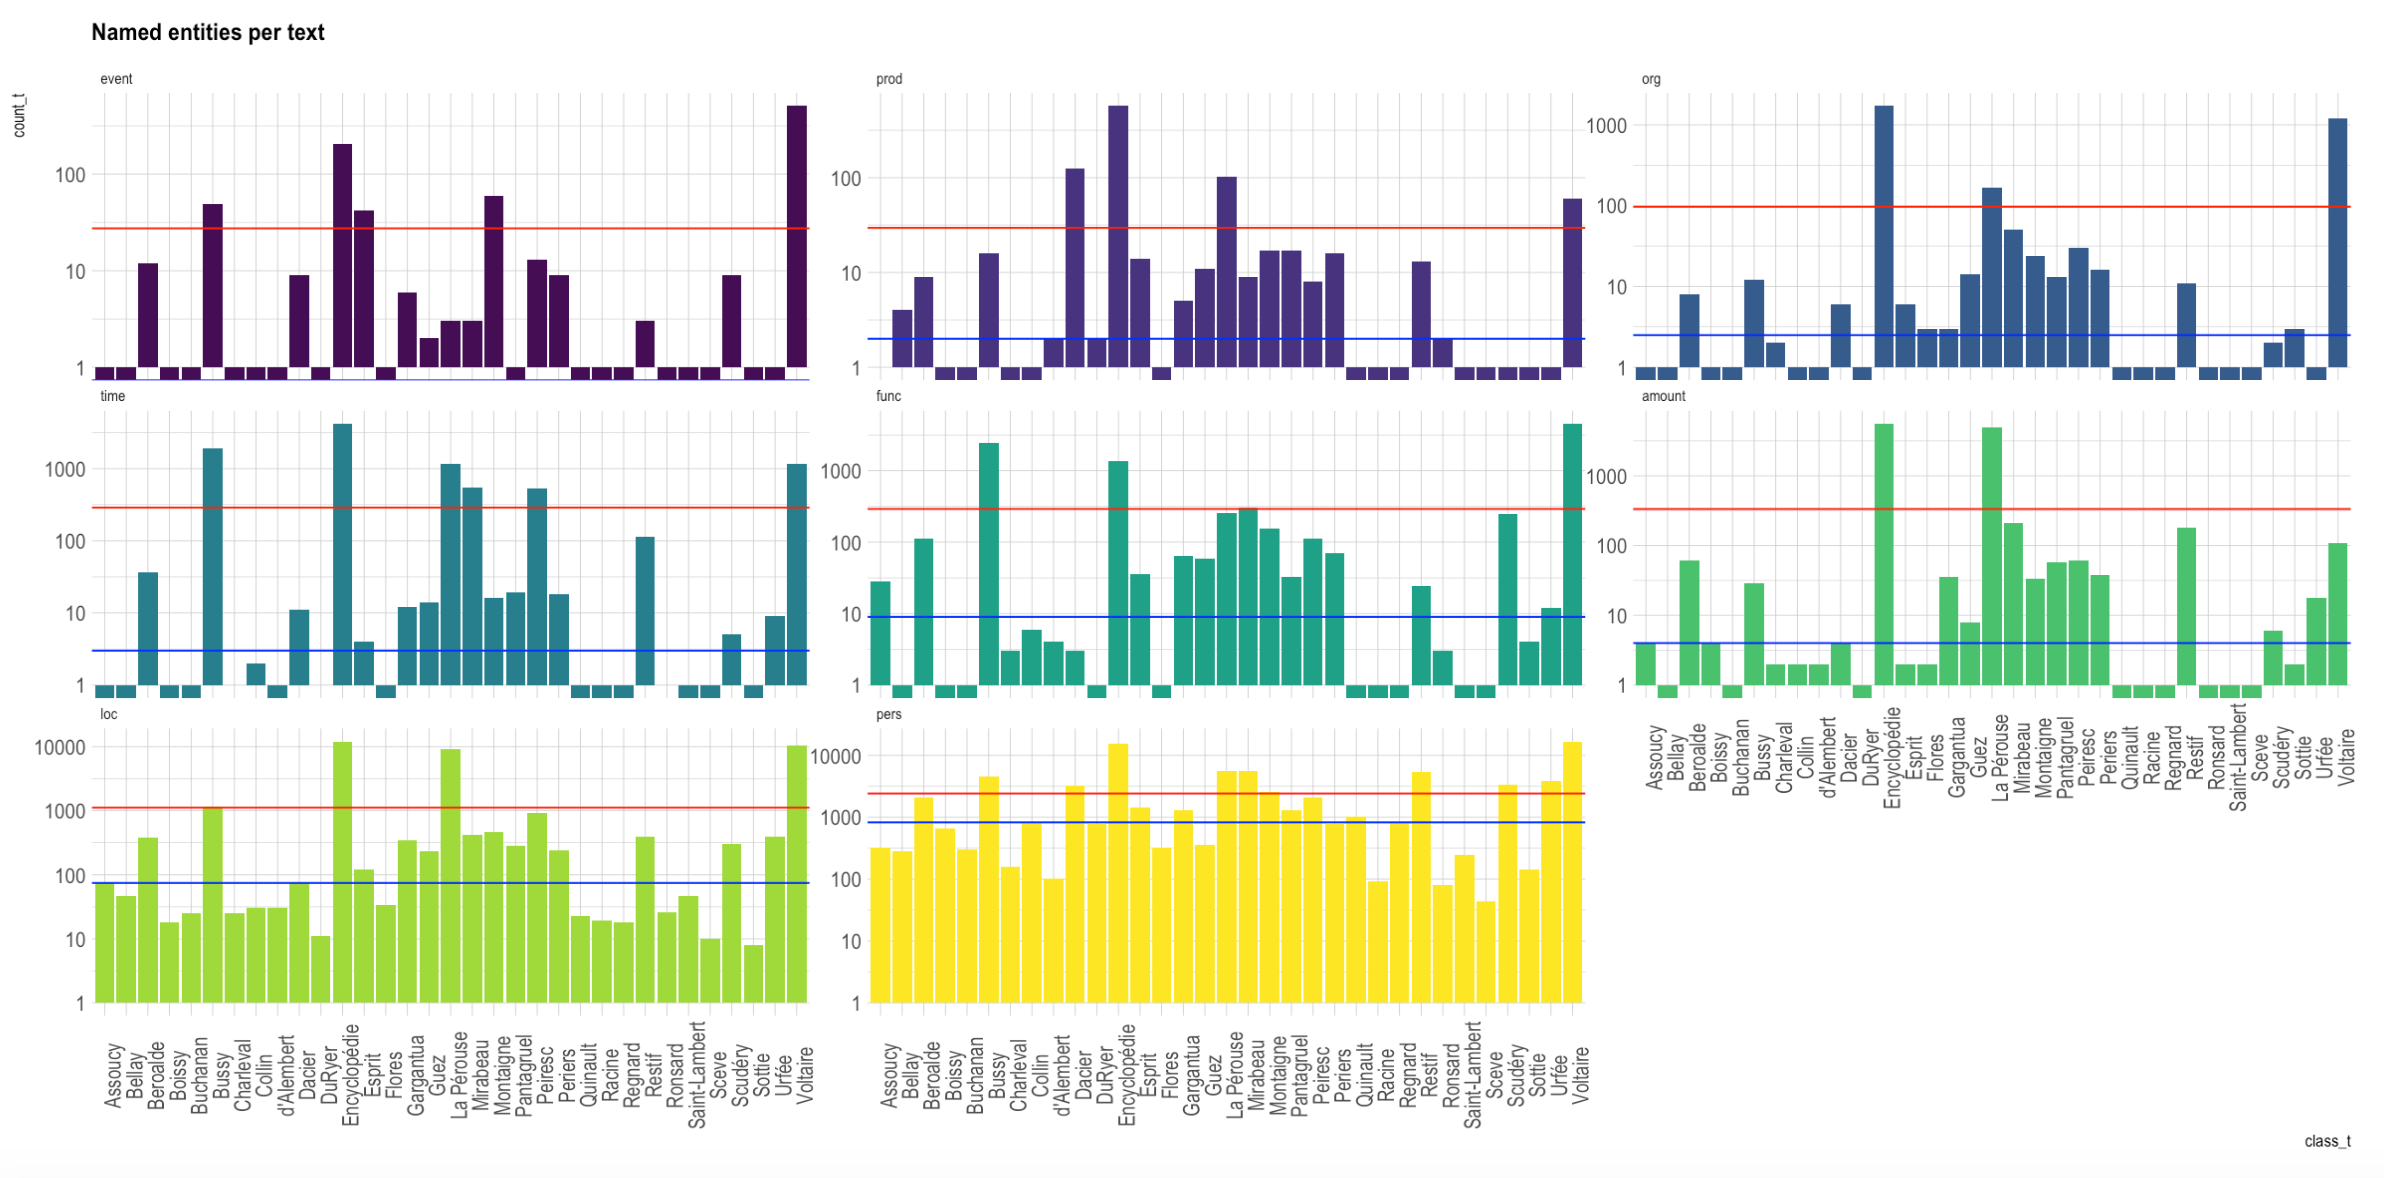
\includegraphics[width=\textwidth]{static/media/mod_eval/dalembert/freem_ner_entity_type_by_text.png}
    \caption{Entity types by text on a logarithmic scale.}
    \label{fig:entity-type-per-text}
\end{sidewaysfigure}
